\documentclass[12pt, titlepage]{article}

\usepackage{booktabs}
\usepackage{tabularx}
\usepackage{hyperref}
\usepackage{graphicx}
\usepackage{gensymb}
\hypersetup{
    colorlinks,
    citecolor=black,
    filecolor=black,
    linkcolor=red,
    urlcolor=blue
}
\usepackage[round]{natbib}

%% Comments

\usepackage{color}

\newif\ifcomments\commentstrue

\ifcomments
\newcommand{\authornote}[3]{\textcolor{#1}{[#3 ---#2]}}
\newcommand{\todo}[1]{\textcolor{red}{[TODO: #1]}}
\else
\newcommand{\authornote}[3]{}
\newcommand{\todo}[1]{}
\fi

\newcommand{\wss}[1]{\authornote{blue}{SS}{#1}}
\newcommand{\an}[1]{\authornote{magenta}{Author}{#1}}

\newcommand{\progname}{Tamias2D}

\begin{document}

\title{Test Report: \progname A 2D Rigid Body Game Physics Library} 
\author{Oluwaseun Owojaiye}
\date{\today}
	
\maketitle

\pagenumbering{roman}

\section{Revision History}

\begin{tabularx}{\textwidth}{p{3cm}p{2cm}X}
\toprule {\bf Date} & {\bf Version} & {\bf Notes}\\
\midrule
Dec. 12, 2018 & 1.0 & Initial draft\\
Dec. 24, 2018 & 1.1 & Updates throughout document\\
\bottomrule
\end{tabularx}

~\newpage

\section{Symbols, Abbreviations and Acronyms}


%\wss{symbols, abbreviations or acronyms -- you can reference the SRS tables if needed}
The symbols, abbreviations, and acronyms used in this document include those defined in the table below, as well as any defined in the tables found in Section 2 of the Software Requirements Specification (SRS) at
\url {https://github.com/smiths/caseStudies/blob/gamephy_finaldoc/CaseStudies/gamephys/docs/SRS/GamePhysicsSRS.pdf}

~\newline
\renewcommand{\arraystretch}{1.2}

\begin{tabular}{l l} 
	
	\toprule		
	
	\textbf{symbol} & \textbf{description}\\
	
	\midrule
	
	MIS & Module Interface Specification\\
	
	MG & Module Guide\\
	
	TC & Test Case\\
	
	VnV & Verification and Validation\\
	
	\bottomrule
	
\end{tabular}\\
\newpage

\tableofcontents

\listoftables %if appropriate

\listoffigures %if appropriate

\newpage

\pagenumbering{arabic}

This document outlines the results of testing for \progname{}. Evaluation of Functional and Non Functional Requirements testing are reported in Sections 2 and 3 respectively. This document is related to the System VnV plan and should be referenced when reviewing this document for the details of System VnV test cases. System VnV Plan document can be found at \url{https://github.com/smiths/caseStudies/blob/gamephy_finaldoc/CaseStudies/gamephys/docs/VnVPlan/SystVnVPlan/SystVnVPlan.pdf}. I did some comparison with an existing library Pymunk, although just one or two scenarios were compared and my findings are reported in section 5. All changes made as a result of changes to requirement(if any), bug fixes and error detection were discussed in section 7. Section 8 describes the test framework used for test automation. Section 9 and 10 details the traceability between test cases, requirements and modules.
were implemented with an automated testing framework. 

\section{Functional Requirements Evaluation}
All functional requirement test cases executed as a part of the System VnV can be found in section 5.1. TC1-TC7 tests for the movement of a body when force or no force is applied and the history of the position and velocity of rigid bodies over time is recorded. This set of test cases cover the functional requirements to create a space for all rigid body simulation(R1), the bodies were initialized with initial values and no force or force was applied on the rigid bodies, the inputs set for the parameters were also verified (R4)and the position and velocities over a period of time was computed upon a force acting on a body (R5).

TC8 - TC9 verified the rotational motion of a body when a rotational force known as 'torque' acts on the body. The angular orientation and angular velocities are computed over a period of time and this satisfies R6. 

T10 - T11 verifies the collision of rigid bodies, in collision test, the software checks for collision, i.e if 2 objects are intersecting and occupying the same position in space(R7) and the collision response is also computed by the software,Coefficient of restitution is applied in collision of 2 objects(R3) and the position and velocities over a period of time is also computed(R8).
All the above test cases passed.

\section{Nonfunctional Requirements Evaluation}

\subsection{Performance}
The performance of \progname{} was tested by stress test, using TC9 of the System VnV Plan, 50 dynamic rigid bodies were added to space and we compute the velocity and position of each body over 4 seconds. The system was able to return all the position and velocity output of all 50 bodies without crashing or slowing down. It took 38.35 secs to return all values.
This result will be compared to Pymunk in a future phase.
The graph below illustrates the output of performance test.
\olu{I had a hard time capturing the legend in one screen}
\begin{figure}[htbp]
	
	\begin{center}
		
		{
			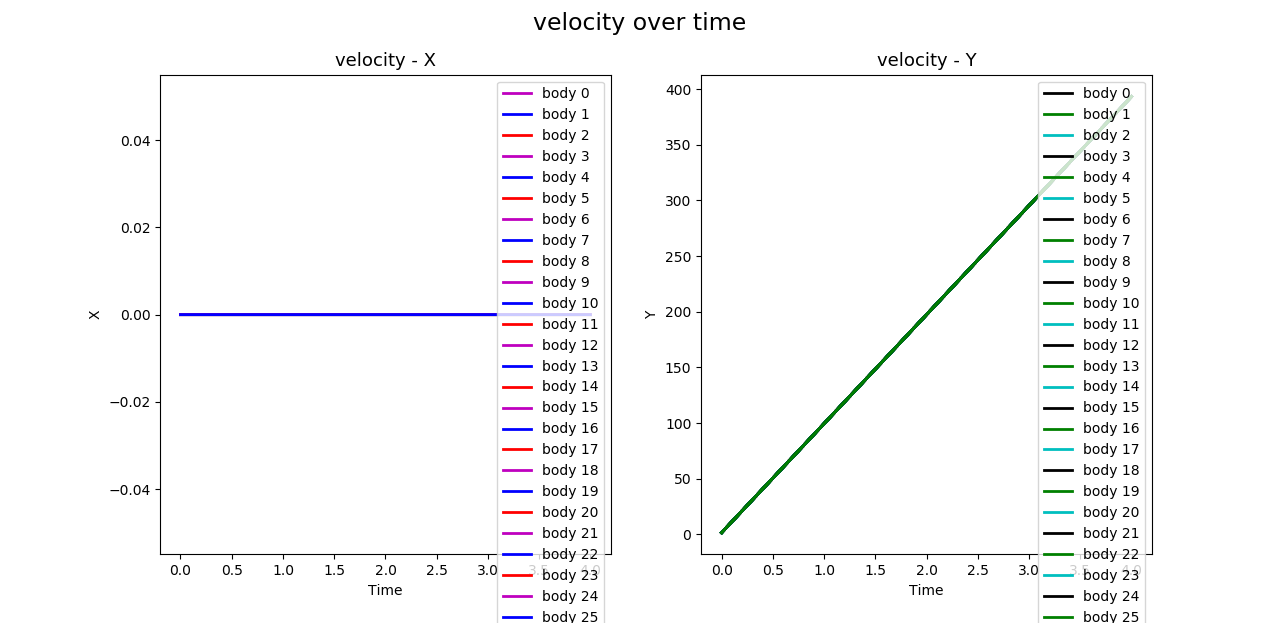
\includegraphics[width=0.71\textwidth]{stresstest.png}
			
		} 
		\caption{\label{Fig_stress}Output Performance of \progname{}}
		
	\end{center}
	
\end{figure}


	
\subsection{Correctness}
The NFR of correctness was measured by comparing actual simulation results of the velocity and position history of \progname with the expected result and the relative error is shown in the image below. TC2 results are displayed. The results give more confidence to the correctness of \progname
~\newline
\begin{figure}[htbp]
	
	\begin{center}
		
{
		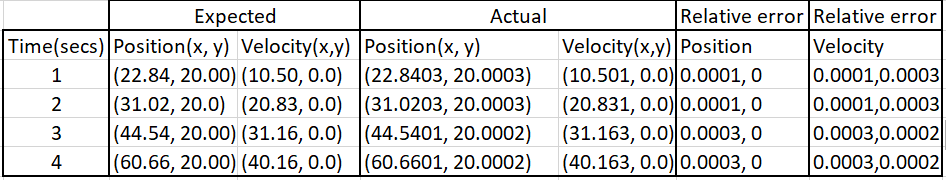
\includegraphics[width=0.71\textwidth]{OutputTC1.png}
			
} 
		\caption{\label{Fig_stresstest}Output Correctness of \progname{}}
		
	\end{center}
	
\end{figure}

Figure 3 shows the output result of a simulation of projectile motion. The object was launched at an angle of $60\degree$. Figures 3 and 4 respectively show the position-time graph and the velocity-time graph. With a trend of the velocity decreasing on the y-axis and constant in the x-axis and change in position forming a projectile pattern, I deduce that the computation is correct as the expected results matches the actual results.
\begin{figure}[htbp]
	
	\begin{center}
		
		{
			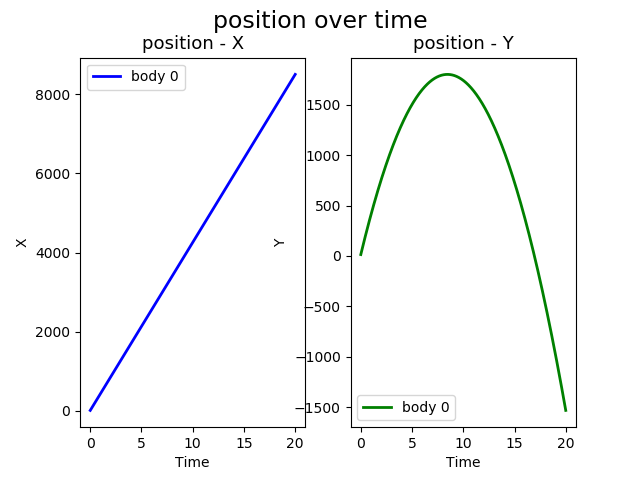
\includegraphics[width=0.71\textwidth]{projectile_60p.png}
			
		} 
		\caption{\label{Fig_projectile_60p}Change in position for projectile motion test \progname{}}
		
	\end{center}
	
\end{figure}

\begin{figure}[htbp]
	
	\begin{center}
		
		{
			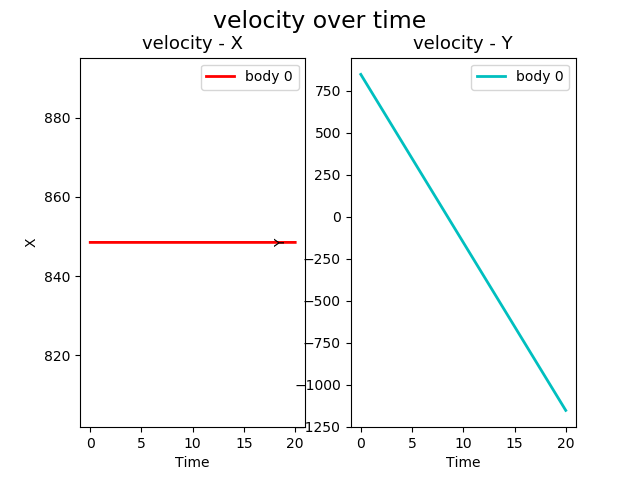
\includegraphics[width=0.71\textwidth]{projectile_60v.png}
			
		} 
		\caption{\label{Fig_projectile_60v}Change in velocity for projectile motion test \progname{}}
		
	\end{center}
	
\end{figure}
~\newpage
\subsection{Usability}
Usability was evaluated by how long it took a user to create a small program as per NFR TC12. After the software was downloaded, the user which was me,I was able to create a program to simulate the movement of 2 rigid bodies in space, computing their velocity and position over time in about 9.22 minutes, so an intermediate to experienced programmer especially one who is familiar with using game physics library will be able to do this in about 20 to 35 minutes and a programmer new to game development might take no less than 1 hour to create the small program described above. This proves the usability of \progname{}
	
\section{Comparison to Existing Implementation}	
\progname was compared with Pymunk for TC1 and TC2, please refer to tables 1 and 2 for results,the result shows that \progname output result of TC1 and TC2 matches the output result of Pymunk. More testing will be done in a later phase of this project. Pymunk will continually be used as a benchmark for \progname
This section will not be appropriate for every project.

\section{Unit Testing}
Please refer to the Unit VnV document located at \url{https://github.com/smiths/caseStudies/blob/gamephy_finaldoc/CaseStudies/gamephys/docs/VnVReport/UnitVnVReport/UnitVnVReport.pdf} for a detailed report on Unit VnV testing.

\section{Changes Due to Testing}
No changes were made due to testing. All tests were successfully executed.

\section{Automated Testing}
Pytest framework was used for automated testing. Please refer to test file located at 
		
\section{Trace to Requirements}
The table below shows the traceability between the test cases in 
the System V\&V Plan and the requirements

\begin{table} [h!]
	
	\centering
	
	\begin{tabular}{|c|c|}
		
		\hline	
		
		\textbf{T} & \textbf{Requirements}\\
		
		\hline 
		
		TC1-TC7& R1, R2, R4, R5\\ \hline 
		TC8-TC9& R1, R2, R4, R5\\ \hline
		TC10-TC11& R1, R3, R4, R7, R8\\ \hline
		TC12& R1, R3, R4, R7, R8\\ \hline
		TC13& R1, R3, R4, R7, R8\\ \hline
		TC14& R1, R3, R4, R7, R8\\ \hline
	\end{tabular}
	
	\caption{Traceability Between Test Cases and Requirements}
	
	\label{Table:Traceability} 
	
\end{table}
 ~\newpage		
\section{Trace to Modules}	

\begin{table} [h!]
	
	\centering
	
	\begin{tabular}{|c|c|}
		
		\hline	
		
		\textbf{T} & \textbf{Modules}\\
		
		\hline 
		
		TC1-TC7& Body, Space, Vector\\ \hline 
		TC8-TC9& Body, Space, Vector\\ \hline
		TC10-TC11& Body, Space, Vector, Shape, Collision Solver\\ \hline
		\end{tabular}
	
	\caption{Traceability Between Test Cases and Modules}
		
\end{table}	

\section{Code Coverage Metrics}
Not Applicable
\bibliographystyle{plainnat}

\bibliography{SRS}

\end{document}